%%%%%%%%%%%%%%%%%%%%%%% file template.tex %%%%%%%%%%%%%%%%%%%%%%%%%
%
% This is a general template file for the LaTeX package SVJour3
% for Springer journals.          Springer Heidelberg 2010/09/16
%
% Copy it to a new file with a new name and use it as the basis
% for your article. Delete % signs as needed.
%
% This template includes a few options for different layouts and
% content for various journals. Please consult a previous issue of
% your journal as needed.
%
%%%%%%%%%%%%%%%%%%%%%%%%%%%%%%%%%%%%%%%%%%%%%%%%%%%%%%%%%%%%%%%%%%%
%
% First comes an example EPS file -- just ignore it and
% proceed on the \documentclass line
% your LaTeX will extract the file if required
\begin{filecontents*}{example.eps}
%!PS-Adobe-3.0 EPSF-3.0
%%BoundingBox: 19 19 221 221
%%CreationDate: Mon Sep 29 1997
%%Creator: programmed by hand (JK)
%%EndComments
gsave
newpath
  20 20 moveto
  20 220 lineto
  220 220 lineto
  220 20 lineto
closepath
2 setlinewidth
gsave
  .4 setgray fill
grestore
stroke
grestore
\end{filecontents*}
%
\RequirePackage{fix-cm}
%
%\documentclass{svjour3}                     % onecolumn (standard format)
%\documentclass[smallcondensed]{svjour3}     % onecolumn (ditto)
\documentclass[smallextended]{svjour3}       % onecolumn (second format)
%\documentclass[twocolumn]{svjour3}          % twocolumn
%
\smartqed  % flush right qed marks, e.g. at end of proof
%
\usepackage{graphicx,amsfonts,amssymb,amsmath}
\usepackage[linesnumbered,ruled]{algorithm2e}
% \usepackage{mathptmx}      % use Times fonts if available on your TeX system
%
% insert here the call for the packages your document requires
%\usepackage{latexsym}
% etc.
%
% please place your own definitions here and don't use \def but
% \newcommand{}{}
%
% Insert the name of "your journal" with
% \journalname{myjournal}

\DeclareMathOperator{\cone}{cone}
\DeclareMathOperator{\inte}{int}
\DeclareMathOperator{\Tol}{Tol}
\DeclareMathOperator{\aff}{aff}
\DeclareMathOperator{\icore}{icore}
\DeclareMathOperator{\bdr}{bdr}
\DeclareMathOperator{\diag}{diag}
\DeclareMathOperator{\sgn}{sgn}
\DeclareMathOperator{\grad}{grad}
\DeclareMathOperator{\Hess}{Hess}
\DeclareMathOperator{\sym}{sym}
\DeclareMathOperator{\cond}{cond}

\newcommand{\p}{\partial}
\newcommand{\lng}{\langle}
\newcommand{\rng}{\rangle}
\newcommand{\lf}{\left}
\newcommand{\rg}{\right}
\newcommand{\sa}{\sqcap}
\newcommand{\su}{\sqcup}
\newcommand{\R}{\mathbb{M}athbb R}
\newcommand{\N}{\mathbb{M}athbb N}
\newcommand{\T} { \rm T}
\newcommand{\Q}{\mathbb{M}athbb Q}
\newcommand{\f}{\frac}
\newcommand{\ds}{\displaystyle}
\newcommand{\m}{\mathbb{M}}
\newcommand{\tpm}{T_{p}\mathbb{M}}
\newcommand{\tpms}{T_{p_*}\mathbb{M}}
\newcommand{\mbg}{\mbox{grad}\,f}
\newcommand{\mbh}{\mbox{Hess}\,f}
\newcommand{\trace}{\,\mbox{trace}\,}

\newcommand\mycommfont[1]{\footnotesize\ttfamily\textcolor{blue}{#1}}
\SetCommentSty{mycommfont}
\SetKwInput{KwInput}{Input}                % Set the Input
\SetKwInput{KwOutput}{Output}              % set the Output


\begin{document}

\title{A modified Armijo for damping a Riemannian Newton-type method}
%\thanks{Grants or other notes
%about the article that should go on the front page should be
%placed here. General acknowledgments should be placed at the end of the article.}

%\subtitle{Do you have a subtitle?\\ If so, write it here}

%\titlerunning{Short form of title}        % if too long for running head

\author{Marcio Ant\^onio de Andrade Bortoloti         \and
        Teles Ara\'ujo Fernandes %etc.
}

%\authorrunning{Short form of author list} % if too long for running head



\institute{Marcio Ant\^onio de Andrade Bortoloti \at
	DCET/UESB, CP-95, CEP 45083-900-Vit\'oria da Conquista, Bahia, Brazil \\
	\email{mbortoloti@uesb.edu.br}           %  \\
	%             \emph{Present address:} of F. Author  %  if needed
	\and
	Teles Ara\'ujo Fernandes \at
	DCET/UESB, CP-95, CEP 45083-900-Vit\'oria da Conquista, Bahia, Brazil \\
	\email{telesfernandes@uesb.edu.br} 
}

\date{Received: date / Accepted: date}
% The correct dates will be entered by the editor


\maketitle

\begin{abstract}
In this work, we present a strategy of linesearch to find singularities of vector fields defined on Riemannian manifolds. We adapt the Armijo rule for preventing a too small step length on the Newton direction, when it exists. Otherwise, we keep the Armijo rule on a safeguard direction. This strategy improves the damped Riemannian Newton method.
We employ the proposed algorithm to minimize a joint diagonalization problem on the Stiefel manifold, and to find singularities of a non-conservative vector field on the sphere.
Our numerical study shows the presented strategy has a good performance.
\keywords{Armijo linesearch \and Global convergence \and Riemannian Newton method}
% \PACS{PACS code1 \and PACS code2 \and more}
\subclass{90C30 \and 49M15  \and 65K05}
\end{abstract}



\section{Introduction}
\label{Introduction}
In this work, we propose an adapted Armijo linesearch for globalizing Newton method, to find a point $p\in\mathbb{M}$ satisfying
\begin{equation}\label{Eq:MainProblem}
X(p)=0,
\end{equation}
where $X:\mathbb{M}\to T\mathbb{M}$ is a differentiable vector field, $\mathbb{M}$ is a finite dimensional Riemannian manifold, and $T\m$ is  the tangent bundle of $\m$. Notice that finding singularities of gradient vector fields on Riemannian manifolds,  which includes finding local minimizers, is a particular case to problem \eqref{Eq:MainProblem}. 

\noindent {\bf In the 1970s, or earlier, iterative methods on manifolds arise in the context of optimizing a real-valued function (see \cite{Luenberger1972}).} In recent years, there has been a growing interest for the development of numerical algorithms for manifolds, see  \cite{bortoloti2022efficient,sato2021}.
%Around the 1990s, the main research issue was to exploit differential-geometric objects in order to formulate optimization strategies on abstract nonlinear manifolds, see \cite{Gabay1982,EdelmanAriasSmith1999}.
There are many numerical problems posed in manifolds arising in various natural contexts, for instance, finding the largest eigenvalue of a symmetric matrix may be posed as maximizing Rayleigh's quotient defined on a sphere, invariant subspace computations, and matrix diagonalization problems.
These problems may be naturally posed on Riemannian manifolds.
Hence, we can use the specific underlying geometric and algebraic structures to reduce significantly the computational cost of finding the zeros of a vector field.
{\bf It is well-known that Newton's method generetes a sequence that converges quadratically to a zero of a vector field. However, it a local convergence, by nature. In other words, Newton's method will converge to the zero of a vector field, when provided it a good enough starting guess, see \cite{Ortega1990,Absil2009,Ferreira2012,FernandesAndFerreiraAndYuan2017}. Unfortunately, it is usual to expend significant computational effort to obtain a good enough starting guess. To overcome this drawback of Newton's method for \eqref{Eq:MainProblem}, a strategy have been introduced is to combine Newton's method with global methods for unconstrained optimization to produce a global method for \eqref{Eq:MainProblem}, (see \cite{MR4102428}).}
In cases where the objective function is twice continuously differentiable and strictly convex, the Newton direction is a descent one of the objective function.
As a consequence, by adjusting the step size in the Newton direction using the Armijo rule, for instance, we can ensure global convergence of this method.
This is a strategy of dumping the Newton step size to globalize this method which  is known as damped Newton's method, see \cite{Dennis1996,Bertsekas2014,Burdakov1980}.
For a recent study, see \cite{bortoloti2022efficient,MR4102428}. {\bf It is well-known that, if the Newton direction is not generated by selecting a starting point close to a solution, the step length, obtained by Armijo linesearch, may be quite small.}
To fix this issue, in this paper we present an adapted Armijo linesearch in order to produce a satisfactory step length on the Newton direction, when it exists.
Otherwise, we keep the classical Armijo linesearch on a safeguard direction for preventing the premature stopping of algorithm.
\vspace{0.2cm}

{\bf SERÁ ALTERADO APÓS NOVA SEÇÃO:} To analyze the numerical behavior of the proposed algorithm, we have considered problems on Stiefel and sphere manifolds.
 The results show that the proposed algorithm has a good performance when compared with Algorithm 3 presented in \cite{bortoloti2022efficient}.



The remainder of this paper is organized as follows. In the next section, we present some basic concepts and preliminary results, Section \ref{sec:DampedNewtonMethod1} presents the main algorithm and a convergence analysis. In Section \ref{Sec:Numerical_Experiment}, numerical experiments are presented, and finally, we conclude this paper with some comments.

\section{Preliminaries}\label{sec:basic}
In this section, we briefly introduce notations, definitions, and auxiliary results we will use in the rest of the paper. Some basic concepts used here can be found in many introductory books on Riemannian geometry, for example, \cite{doCarmo1992,Sakai1996}.
We denote $\mathbb{M}$ as a {\it finite dimensional Riemannian manifold},
$\tpm$ the {\it tangent space} of $\m$ at $p$, and $T\m=\bigcup_{p\in\m}\tpm$ the {\it tangent bundle} of $\m$.
The corresponding norm associated to the Riemannian metric $\langle \cdot ~, ~ \cdot \rangle$ is denoted by $\|  \cdot \|$. We denote $\|\cdot\|_F$ as the Frobenious norm. The Riemannian  distance  between $p$ and $q$ in $\mathbb{M}$ is given  by $d(p,q)$,  which induces the original topology on $\mathbb{M}$, namely,  $(\mathbb{M}, d)$ that represents a complete metric space.   The open ball of radius $r>0$ centred at $p$ is defined as  $B_{r}(p):=\left\lbrace q\in\m:d(p,q)<r\right\rbrace$.  Let  $\Omega \subseteq   \m$ be an open set and denote by ${\cal X}(\Omega)$ the {\it space of  differentiable  vector fields} on $\Omega$.  Let $\nabla$ be the Levi-Civita connection associated to $(\mathbb{M}, \langle \cdot ~, ~ \cdot \rangle)$.  The covariant derivative of $X \in {\cal X}(\Omega)$, determined by $\nabla$, defines at each $p\in \Omega$ a linear map $\nabla X(p):\tpm\to\tpm$ given by $\nabla X(p)v=\nabla_{Y}X(p),$
where $Y$ is a vector field such that $Y(p)=v$.
For $f: \mathbb{M} \to \mathbb{R}$ a twice-differentiable function, the Riemannian metric, induces the mappings $f\mapsto  \mbox{grad} f $ and   $f\mapsto \mbox{Hess} f$. Its {\it gradient} and {\it hessian} can be associated to the Riemannian metric by
\begin{equation}\nonumber
\langle \mbox{grad} f,X\rangle:=d f(X),  \qquad    \langle \mbox{Hess} f X,X\rangle :=d^2 f(X, X),  \qquad \forall~ X \in {\cal X}(\Omega),
\end{equation}
respectively. The last two equalities imply  $\mbox{Hess} f X= \nabla_{X}  \mbox{grad} f$,   for all  $X \in {\cal X}(\Omega)$.
The {\it norm of a  linear map} $A:T_p \mathbb{M} \to T_p \mathbb{M}$  is defined by $\|A\|:=\sup \left\{ \|Av \|~:~ v\in T_p \mathbb{M}, \,\|v\|=1 \right\}$.  A vector field $V$ along a differentiable curve $\gamma$ in $\mathbb{M}$ is said to be {\it parallel} iff $\nabla_{\gamma^{\prime}} V=0$.  For each $t \in [a,b]$, the operator $\nabla$ induces an isometry relative to Riemannian metric $ \langle \cdot , \cdot \rangle  $, $P_{\gamma,a,t} \colon T _{\gamma(a)} {\mathbb{M}} \to T _{\gamma(t)} {\mathbb{M}}$, defined by $ P_{\gamma,a,t}\, v = V(t)$, where $V$ is the unique vector field on $\gamma$ such that
$\nabla_{\gamma'(t)}V(t) = 0$ and $V(a)=v$. Further, we can notice $ P_{\gamma,\,b_{1},\,b_{2}}\circ P_{\gamma,\,a,\,b_{1}}=P_{\gamma,\,a,\,b_{2}}$ and  $P_{\gamma,\,b,\,a}=P^{-1}_{\gamma,\,a,\,b}$. As long as there is no confusion, we will  consider the notation $P_{pq}$  instead of $P_{\gamma,\,a,\,b}$, when $\gamma$ is the unique segment of curve joining  $p$ and $q$. In the next, we present a function which is used to establish the proposed algorithm.

\begin{definition}\label{eq:MeritFunction}
Let $X:\mathbb{M}\to T\mathbb{M}$ be a differentiable vector field. The merit function is defined by
\begin{equation}\label{Eq:meritfanction}
\varphi(p)=\dfrac{1}{2}\|X(p)\|^{2}.
\end{equation}
\end{definition}
\noindent The next definition introduces the concept of retraction, which has been introduced by \cite{Manton2002}. It is a generalization of the classical exponential mapping.
\begin{definition}\label{Df:nqc}
A \textit{retraction} on a manifold $\mathbb{M}$ is a smooth mapping $R$ defined from the tangent bundle $T\mathbb{M}$ onto $\mathbb{M}$ with the following properties: If $R_{p}$ denotes the restriction of $R$ to $T_{p}\mathbb{M}$, then
\begin{itemize}
\item[(i)] $R_{p}(0_{p})=p$, where $0_{p}$ denotes the origin of $T_{p}\mathbb{M}$;
\item[(ii)] With the canonical identification $T_{0_{p}}T_{p}\mathbb{M}\simeq T_{p}\mathbb{M}$, $R'_{p}(0_{p})=I_{p}$, where $I_{p}$ is the identity mapping on $T_{p}\mathbb{M}$, and $R'_{p}$ denotes the diferential of $R_{p}$.
\end{itemize}
\end{definition}

\begin{remark}
Since $R'_{p}(0_{p})=I_{p}$, by the Inverse Function Theorem, $R_{p}$ is a local diffeomorphism (see \cite[Cap. 2, Sec. 2]{Sakai1996}). Hence, we can define the {\it injectivity radius} of $\mathbb{M}$ at $p$ with respect to $R$ by 
$$i_{p}:=\sup\left\{ r>0~:~{R_{p}}_{\lvert_{B_{r}(0_{p})}} \mbox{ is\, a\, diffeomorphism} \right\},$$
where $B_r(0_{p}):=\left\lbrace  v\in T_{p}\mathbb{M}:\parallel v-0_{p}\parallel <r\right\rbrace$. In case $\bar{p}\in \mathbb{M}$. Then the above definition implies  that if we consider $\delta$ such that $0<\delta<i_{\bar{p}}$, then $V_{\delta}( \bar p):=R_{\bar p}B_{\delta}(0_{ \bar p})$ is an open set. Moreover, for all $p\in V_{\delta}( \bar p)$  the  curve segment $\gamma_{\bar{p}p}(t)=R_{\bar{p}}\left(t R^{-1}_{\bar p}p\right)$ joining  $\bar p$ to $p$ belongs to $V_{\delta}( \bar p)$.
\end{remark}


\noindent The first auxiliary result of this work establishes that,  if $\nabla X(\bar{p})$ is nonsingular then there exists a neighborhood of $\bar{p}$ such that $\nabla X$ is also nonsingular. Its proof can be found in \cite[Lemma 3.2]{FernandesAndFerreiraAndYuan2017}.

\begin{lemma}\label{le:NonSing}
Consider that $\nabla X$ is a continuous operator at ${\bar p} \in \mathbb{M}$. Then, ${\lim_{p\to {\bar p}}}\left \| P_{p{\bar p}}\nabla X(p)P_{{\bar p}p}-\nabla X({\bar p}) \right \|=0.$ Moreover, if $\nabla X({\bar p})$ is  nonsingular then there exists  $0<\delta<\delta_{{\bar p}}$ such that, for each $p\in B_{\delta}({\bar p})$,   $\nabla X(p)$ is nonsingular and $\left \| \nabla X(p)^{-1}\right \|\leq 2\left \|\nabla X({\bar p})^{-1}\right \|$.
\end{lemma}
\noindent Consider the constant value $\delta$ given by Lemma~\ref{le:NonSing}. Denote $\bar{\delta}:=\delta$, $R$ a retraction, and $X$ a differentiable vector field. We define {\it Newton's iterate mapping} as follows:
\begin{eqnarray*}
N_{R,X}:B_{\bar{\delta}}(\bar{p}) &\to&  \mathbb{M}\\
p&\mapsto&R_{p}(-\nabla X(p)^{-1}X(p)).
\end{eqnarray*}

%The existence  of a neighborhood of $\bar{p}$ where Newton's iterate \eqref{Newton's iterate mapping} belong to the same neighborhood is established by following lemma, see \cite[Lemma 3]{bortolotiandfernandesandferreira}.
%\begin{lemma}\label{L:InvNx}
%Let  $\bar{p}\in\mathbb{M}$ such that $X(\bar p)=0$. If $\nabla X$ is continuous at $\bar p$ and $\nabla X(\bar{p})$ is nonsingular,  then  there exists $0<\hat{\delta}<\delta_{\bar{p}}$ such that $B_{\hat{\delta}}(\bar{p})\subset \Omega$ and $\nabla X(p)$ is nonsingular  for each $p\in B_{\hat{\delta}}(\bar{p})$. Moreover,    $N_{R,X}(p)\in B_{\hat{\delta}}(\bar{p})$, for all $p\in B_{\hat{\delta}}(\bar{p})$.
%\end{lemma}

\begin{lemma}\label{Le:SupLinConPhi}
Let  $\bar{p}\in \Omega$ such that $X(\bar p)=0$.  If $\nabla X$ is continuous at $\bar p$ and $\nabla X(\bar p)$ is nonsingular,  then  there exists $0<\hat{\delta}<\delta_{\bar{p}}$ such that, $\nabla X(p)$ is nonsingular  for each $p\in B_{\hat{\delta}}(\bar{p}) \subset \Omega$ and $\lim_{p\to \bar p}\varphi\left(N_{R,X}(p)\right)/\parallel X(p)\parallel^{2}=0$. As a consequence, there is a $\delta>0$ such that,  for all  $\sigma\in(0,1/2)$ and $\delta< \hat{\delta}$  it holds
\begin{equation}\label{eq:ArmijoCond} \nonumber
\varphi\left(N_{R,X}(p)\right) \leq \varphi\left(p\right)+ \sigma \left\langle\grad\,\varphi(p), -\nabla X(p)^{-1}X(p)\right\rangle, \qquad  \forall~p\in B_{\delta}(\bar{p}).
\end{equation}
\end{lemma}
\begin{proof}
See \cite[Lemma 4.3]{bortoloti2022efficient}.
\end{proof}
\noindent We finish this section with the following result whose proof can be found in \cite[Lemma 4.2]{bortoloti2022efficient}.
\begin{lemma}\label{Le:AdTesteNew}
 If $\nabla X$ is continuous at $\bar p\in \Omega$ and $\nabla X(\bar p)$ is nonsingular,  then  there exists $0<\hat{\delta}<\delta_{\bar{p}}$ such that $B_{\hat{\delta}}(\bar{p})\subset \Omega$, $\nabla X(p)$ is nonsingular  for  $p\in B_{\hat{\delta}}(\bar{p})$.  Moreover, for all  $p\in B_{\hat{\delta}}(\bar{p})$  the vector $v=-\nabla X(p)^{-1}X(p)$ is the  unique solution of the linear equation  $X(p)+\nabla X(p)v=0$,   and for $0\leq \theta < 1/\cond (\nabla X(\overline{p}))$  we have
\begin{equation}\label{eq:AdTesteNew} \nonumber
\langle \grad\,\varphi(p), v \rangle \leq -{\theta}\|\grad\, \varphi(p)\| \| v\|, \qquad \forall ~p\in B_{\hat{\delta}}(\bar{p}).
\end{equation}
\end{lemma}


%\begin{remark}
%We would like to point out the $\gamma$ parameter may be estimated by using the condition number of the covariant derivative at solution. However, in some situations, this appears to be not simple. Hence, it is worth employing some effort in order to obtain some useful estimates for practical applications.
%\end{remark}


\section{Globalization of Newton Method}\label{sec:DampedNewtonMethod1}
%%%%%%%%%%%%%%%%%%%%%%%%%%%
In this section, we present an adapted Armijo linesearch to globalize the Newton method to find a point $p\in\mathbb{M}$ satisfying $X(p)=0$, where $X:\mathbb{M}\to T\mathbb{M}$ is a differentiable vector field. In \cite{MR4102428,bortoloti2022efficient}, damped Newton methods were presented to solve this problem. In such works, the idea is to use the Newton method to minimize \eqref{Eq:meritfanction}, taking its gradient as a safeguard direction, when  Newton direction does not exist, and adjusting the step size by using Armijo linesearch for both directions.
Using the same idea, we establish an adapted Armijo linesearch procedure to damping the Newton direction keeping the classical Armijo on safeguard direction. The following algorithm presents formally the strategy.
\begin{algorithm}[H] \label{AL:Newton_NewLinesearch}
\DontPrintSemicolon
  \KwInput{$\sigma \in (0,1/2)$, $\theta \in [0,\gamma)$, $\alpha_{min}>0$, and $p_0 \in \mathbb{M}$.}
  Set $k := 0$.\;
  Compute $v_k \in T_{p_k}M$ such that
  \begin{equation}\label{eq:Newton0}
  X(p_k)+\nabla X(p_k)v_k=0.
  \end{equation} \;
  If  $v_k$ exists, compute
  \begin{equation}\label{eq:passo_Newton}
  \alpha_k:=\max \left\{ 2^{-j}:\varphi\left(R_{p_k}(2^{-j} v_{k})\right)\leq (1+\sigma\theta2^{1-j})\varphi\left(p_{k}\right), j\in \mathbb{N} \right\}.
  \end{equation}
  Otherwise, go to $5$. \;
  If $\alpha_k \ge \alpha_{min}$ go to $6$. \;
  Set the search direction as
  \begin{equation}\label{Eq:safeguardDirection}
    v_{k}=  -\grad\,\varphi(p_{k})=-\nabla X(p_{k})^{*}X(p_{k})
  \end{equation}
  and compute the step size by the rule
  \begin{equation}\label{eq:armijo1}
  \alpha_k:=\max \left\{ 2^{-j}~: ~\varphi\left(R_{p_k}(2^{-j} v_{k})\right)\leq \varphi(p_k)-\sigma 2^{-j}\| \grad\,\varphi(p_k)\|^{2}, ~j\in \mathbb{N} \right\}.
  \end{equation}\;
  Set $p_{k+1} := R_{p_k}(\alpha_k v_k)$.
\caption{ }
\end{algorithm}
\noindent Before presenting our convergence analysis for the proposed algorithm, we describe its characteristics. First, we compute $v_k$ as a solution of  \eqref{eq:Newton0}  if any,  and then we  check if it satisfies \eqref{eq:passo_Newton} for some not too small step length. In this case, we use it as a search direction in {\bf Step 6}. When $v_k$ does not satisfy either \eqref{eq:Newton0} or $\alpha_k\geq\alpha_{min}$ we set $v_{k}=  -\grad\,\varphi(p_{k})$ as the search direction with the Armijo linesearch given by \eqref{eq:armijo1}. Then, we set it to compute the next iterate in {\bf Step 6}. We would like to point out that by Lemma \ref{Le:AdTesteNew}, $\gamma=1/\cond (\nabla X(\overline{p}))$. 

{\bf Nos experimentos numéricos devemos informar como foi obtido o $\gamma$!!!}

The next two results establish properties for  the sequence generated by Algorithm \ref{AL:Newton_NewLinesearch}. The first one assures the existence of the step size on the safeguard direction. Its proof can be found in \cite[Lemma 3]{MR4102428}. The second one assures the existence of the step size on the Newton direction.

%\begin{lemma}\label{L:DescDir}
%Let $p\in \mathbb{M}$ with  $X(p)\neq 0$.  Assume  $v$ is given by \eqref{Eq:safeguardDirection} or is a solution of the  linear equation \eqref{eq:Newton0}. If $v\neq 0$, then $ \left\langle\grad\,\varphi(p),  v\right\rangle <0$ .
%\end{lemma}

\begin{lemma}\label{L:DescDir}
Assume that $p\in \mathbb{M}$ with  $X(p)\neq 0$.  If  $v \neq 0$ is given by \eqref{Eq:safeguardDirection} then $ \left\langle\grad\,\varphi(p),  v\right\rangle <0$ .
\end{lemma}

%\noindent The following result  guarantees that conditions \eqref{eq:Newton0} and \eqref{eq:passo_Newton} are  satisfied in a neighbourhood  of a point where the covariant derivative is nonsingular.

\begin{lemma}\label{lemma:theta}
Let $\bar p\in \Omega\subset\mathbb{M}$ and  $R$ be a retraction. If $\nabla X$ is continuous at $\bar{p}$ and $\nabla X(\bar p)$ is nonsingular then, there exists $0<\hat{\delta}<\delta_{\bar{p}}$ such that $\nabla X(p)$ is nonsingular and the vector $v=-\nabla X(p)^{-1}X(p)$ is the  unique solution of the linear equation  $X(p)+\nabla X(p)v=0$ for all  $p\in B_{\hat{\delta}}(\bar{p})$. Moreover, if $~\varphi$ is given by \eqref{Eq:meritfanction} then, there are $\gamma>0$, $\theta\in[0,\gamma)$, and $\sigma\in(0,1/2)$  such that
\begin{equation}\label{eq:AdTesteNew} \nonumber
 ~\varphi\left(R_{p}(v)\right)\leq (1+2\sigma\theta)\varphi\left(p\right),\qquad\forall p\in B_{\hat{\delta}}(\bar{p}).
\end{equation}
\end{lemma}
\begin{proof}
Since $\nabla X$ is continuous at $\bar p\in \Omega$ and $\nabla X(\bar p)$ is nonsingular, Lemma \ref{le:NonSing} ensures the existence of a $\hat{\delta}$ such that $0<\hat{\delta}<\delta_{\bar{p}}$ and $\nabla X(p)$ is nonsingular  for  each $p\in B_{\hat{\delta}}(\bar{p})$.  Moreover, the vector $v=-\nabla X(p)^{-1}X(p)$ is the  unique solution of the linear equation  $X(p)+\nabla X(p)v=0$, for all  $p\in B_{\hat{\delta}}(\bar{p})$. It follows from Lemma \ref{Le:SupLinConPhi} that
\begin{equation}\nonumber
\varphi\left(R_{p}(v)\right) \leq \varphi\left(p\right)+ \sigma \left\langle\grad\,\varphi(p), v\right\rangle, \qquad  \forall~p\in B_{\hat{\delta}}(\bar{p}).
\end{equation}
 Taking $\gamma = 1/\cond (\nabla X(\overline{p}))$, Lemma \ref{Le:AdTesteNew} ensures that for $\theta\in [0,\gamma)$ we have
\begin{equation}\nonumber
\langle \grad\,\varphi(p), v \rangle \leq -{\theta}\|\grad\, \varphi(p)\| \| v\|, \qquad \forall ~p\in B_{\hat{\delta}}(\bar{p}).
\end{equation}
Moreover, from Cauchy-Schwarz inequality and \eqref{Eq:meritfanction},  we obtain
\begin{equation} \nonumber
-\|\grad\, \varphi(p)\| \| v\|\leq 2\varphi\left(p\right).
\end{equation}
From three last inequalities, we conclude  $\varphi\left(R_{p}(v)\right)\leq (1+2\sigma\theta)\varphi\left(p\right), \forall p\in B_{\hat{\delta}}(\bar{p})$ .
\end{proof}

%\textcolor{red}{\begin{eqnarray}
%\varphi\left(R_{p}(v)\right)&\leq&\varphi\left(p\right)+ \sigma \left\langle\grad\,\varphi(p), v\right\rangle\\
%&\leq&\varphi\left(p\right)-\sigma\theta\|\grad\, \varphi(p)\| \| v\|\\
%&\leq&\varphi\left(p\right)- \sigma\theta \left\langle\grad\,\varphi(p), v\right\rangle\\
%&=&\varphi\left(p\right)+\sigma\theta\|X(p)\|^2\\
%&=&\varphi\left(p\right)+\sigma\theta 2\varphi\left(p\right)\\
%&=&(1+2\sigma\theta)\varphi\left(p\right)\\
%\end{eqnarray}}
%

\noindent We finish this section  by presenting the following theorem which establishes convergence of a sequence generated by Algorithm \ref{AL:Newton_NewLinesearch}. Taking into account Lemma~\ref{lemma:theta}, the proof of this theorem can be made using the same idea in \cite[Theorem 4.2]{bortoloti2022efficient}. For this reason, we do not present it here.

\begin{theorem}\label{theoremAuxiliary123}
Let $\mathbb{M}$ be a Riemannian manifold, $R$ a retraction on $\mathbb{M}$, $X:\mathbb{M} \to T\mathbb{M}$ be a continuously differentiable vector field, and $\left\{p_{k}\right\}$ a sequence generated by Algorithm~\ref{AL:Newton_NewLinesearch}. Then, if $\bar p\in \mathbb{M}$ is an accumulation point of $\left\{p_{k}\right\}$,   $\bar p$ is a critical point of $\varphi$.
Moreover,  if $\nabla X(\bar p)$ is nonsingular, the convergence of $\left\{p_{k}\right\}$ to $\bar p$ is superlinear and $X(\bar p)=0$.
\end{theorem}

\section{Numerical Experiments}\label{Sec:Numerical_Experiment}
%%%%%%%%%%%%%%%%%%%%%%%%%

In this section, we present two examples to show some numerical properties of Algorithm \ref{AL:Newton_NewLinesearch}. The first one is a minimization problem on the Stiefel  manifold that is related to applications in the independent component analysis (ICA).
The second is an academic problem of finding a zero of a non-conservative vector field on the sphere.
We compare the computational performance of Algorithm \ref{AL:Newton_NewLinesearch} with Algorithm 3, proposed in \cite{bortoloti2022efficient}.
All problems were stopped when the norm of vector field reached the tolerance of $10^{-6}$. When on a problem an algorithm has exceeded the maximum number of 2000 iterates we declare it has not been able to solve the problem.
{\bf We have taken the step lengths, given by \eqref{eq:passo_Newton}, always greater than  $\alpha_{min} = 10^{-5}$.}
All Matlab codes are freely available in the following web site: ``https://github.com/mbortoloti/damped-newton-new-linesearch/''.


%%%%%%%%%%%%%%%%%%%%%%%%%%%%%%%%%%%%%%%%%%%%%%%%%%%%%%%%%%%%%%%%%%%%%%%%%%%%%%%%%%%%%%%%%%%%%%%%%%%%%%%%%%%%%%%%%%%%%%%%%%
\subsection{A joint diagonalization problem on the  Stiefel manifold}

We analyse Algorithm \ref{AL:Newton_NewLinesearch} to solve the following joint diagonalization problem defined on the Stiefel manifold:
\begin{problem}\label{pr:diagonalization_onstiefel}
Given $A_1, \cdots,A_N$ symmetric matrices, find $P \in St(n,p)=\{P \in \mathbb{R}^{n \times p}; \, P^TP=I_p\}$, with $p\leq n$, that minimizes
\begin{equation}\nonumber
f(P) = -\sum_{l=1}^N \left\| \diag \Big( P^TA_lP\Big)\right\|_F^2,
\end{equation}
where $\diag(Y)$ is a diagonal matrix generated by the diagonal entries of $Y$.
\end{problem}
\noindent In \cite {MR3734011} was proposed a Newton-type method using a vectorization strategy to solve this problem.
Taking into acount this idea, we implement Algorithm \ref{AL:Newton_NewLinesearch}  and perform numerical experiments considering, for each $l=1, \cdots,N$, the  matrices $A_l=PL_lP^T$, with $P \in St(n,n)$ and $L_l$ a diagonal matrix whose non zero elements are given by $\lambda_1>\cdots>\lambda_n$.
In this case, an optimal  solution is $X^*=PI_{n,p}$, where $I_{n,p}$ is the $n \times p$ identity matrix.
Initial guesses were generated by considering $X_0 = \mbox{qf}(X^*+\rho \; X_{rand})$ where, $X_{rand}$ is a $n \times p$ random matrix and $\rho = 10^{-4}, 10^{-3}, \cdots,10^{2}$.
We assume $N=5$.
For $n=10$ fixed and $p=2,3,4,5$ were considered 10 random initial guesses for each combination of $(n,p)$.
 The sequences were obtained by using the retraction $R_P(V)=\mbox{qf}(P+V)$, where qf denotes the Q factor of QR decomposition.
 We take   $\sigma = 10^{-4}$ and $\theta = 0.9$.
 In Figure \ref{fig:newarmijoxnlse4}, it can be seen that Algorithm \ref{AL:Newton_NewLinesearch} is faster than Algorithm 3 proposed in \cite{bortoloti2022efficient}.
 \begin{figure}[h]
	\centering
	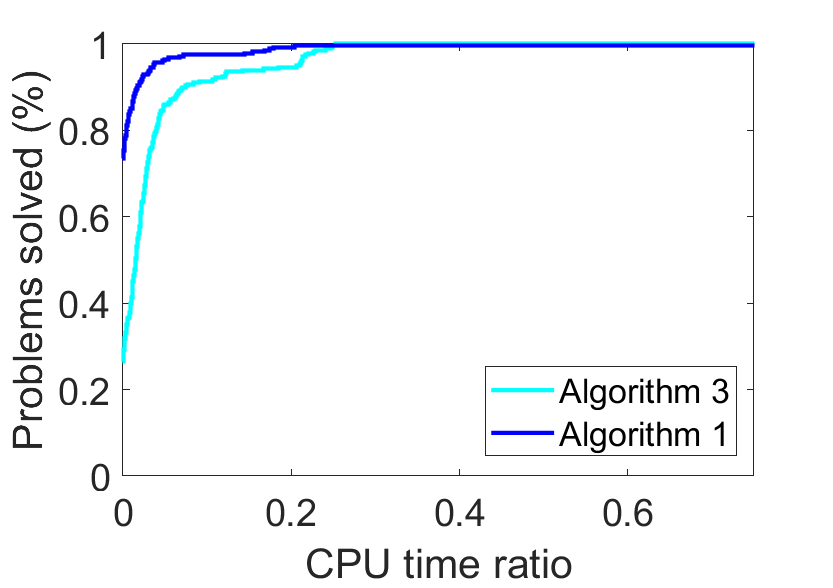
\includegraphics[width=0.6\textwidth]{jointdiag.png}
	\caption{Performance profile comparing the algorithms \ref{AL:Newton_NewLinesearch} and  3 (given in \cite{bortoloti2022efficient}) to solve the Problem \ref{pr:diagonalization_onstiefel}.}
	\label{fig:newarmijoxnlse4}
\end{figure}


\subsection{A Non-Conservative Vector Field on the Sphere}
In this section, we aim to explore the behaviour of Algorithm \ref{AL:Newton_NewLinesearch} applied to find a singularity of a non conservative vector field defined on the sphere. The problem is formally described as the following:

\begin{problem}\label{pr:nonconsevative}
    Find $p \in \mathbb{M}$ such that
    $X(p) = 0$,    where $\mathbb{M}=(S^{n-1},\langle,\rangle)$ is equipped with the canonical metric, $X(p):=Q(p-p^*)-\langle p,Q(p-p^*) \rangle p$ with $Q$ a skew-symmetric matrix, and  a fixed $p^* \in \mathbb{M}$, see \cite{MR4102428}.
\end{problem}

\noindent Numerical study was developed for dimensions $n=100,200,300,400,500$.
 For each dimension, we consider a fixed skew-symmetric matrix $Q=(A-A^T)/2$, where $A$ is a randomly generated matrix.
 It were taken 15 random initial guesses on $\mathbb{M}$, for each dimension, and the parameters of linesearches were $\sigma = 10^{-3}$ and $\theta = 10^{-1}$.
  Performance profiles are depicted on Figure \ref{fig:ncarmxnls} comparing Algorithm \ref{AL:Newton_NewLinesearch} and Algorithm 3, proposed in \cite{bortoloti2022efficient}.
  We can notice Algorithm \ref{AL:Newton_NewLinesearch} solved all problems.
  On the other hand, Algorithm 3 did not solve all problems because the step length became quite small.
  This suggests Algorithm \ref{AL:Newton_NewLinesearch} has contributed to fix this issue.
\begin{figure}
	\centering
	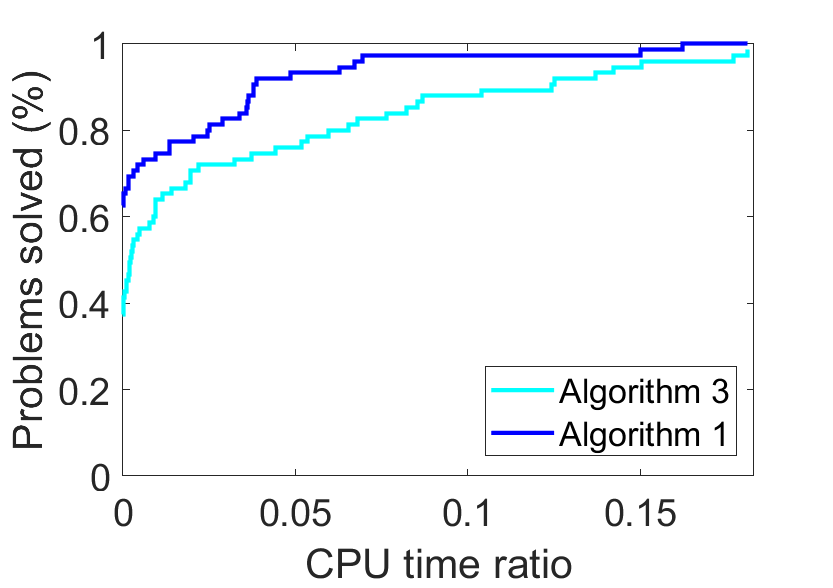
\includegraphics[width=0.6\textwidth]{nonconservative.png}
	\caption{Performance profile comparing the algorithms \ref{AL:Newton_NewLinesearch} and  3  to solve the Problem \ref{pr:nonconsevative}.}
	\label{fig:ncarmxnls}
\end{figure}

\subsection{An academic function on Symmetric Positive Definite Matrices }

Let $ \mathbb{P}^n_{++}$ be the manifold of symmetric positive definite matrices.

\begin{problem}Find $P^* \in \mathbb{P}^n_{++}$, such that $\grad f(P^*) =0$, where $f:\mathbb{P}^n_{++} \to \mathbb{R}$ is given by 
\begin{equation} \label{pr:academicfunction}
f(X) = a \log(\det X) + b \trace (X^{-1}),
\end{equation}
with $a,b > 0$, $\det P$ is the determinant of $P$,   and $\grad f(P)$ is the riemannian gradient of $f$.
\end{problem}


\begin{figure}
	\centering
	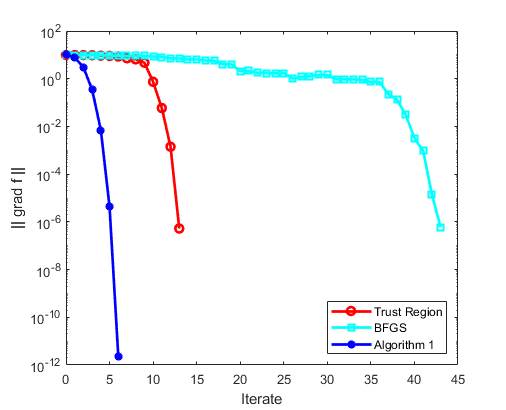
\includegraphics[width=0.6\textwidth]{logdet_iter.png}
	\caption{Iterates.}
	\label{fig:logdetfig}
\end{figure}


\section{ Conclusions} \label{sec:conclusions}
%%%%%%%%%%%%%%%%%%%%%%%%%%
In this work, we have presented a strategy of linesearch to improve the globalization of Riemaniann Newton method, given in \cite{bortoloti2022efficient}.
%In this work, we have presented a strategy to globalize the Newton method in order to find singularities of vector fields defined on Riemannian manifolds.
This strategy relaxes the Armijo rule for preventing a step length quite small on the Newton direction.
From a numerical point of view, we would like to note the step length given in \eqref{eq:passo_Newton} appeared to be sensitive to the inverse of the conditioning number of the covariant derivative of considered vector field. It would be interesting to develop a study to obtain a further improvement of the Algorithm \ref{AL:Newton_NewLinesearch}.
%The proposed method presents a new linesearch, which relaxes the Armijo rule, for preventing a step length quite small on the Newton direction.
%In the cases where this can not be assured we set the classical Armijo linesearch on safeguard direction.
%Since the $\gamma$ parameter, given in Lemma \ref{Le:AdTesteNew}, depends on the condition number of covariant derivative at the solution, it would be interesting a study to obtain a further improvement of the Algorithm \ref{AL:Newton_NewLinesearch}.
Numerical experiments were developed on the Stiefel and sphere manifolds. They show that Algorithm \ref{AL:Newton_NewLinesearch} presents good performance when compared with Algorithm 3 presented in \cite{bortoloti2022efficient}.


%\section{Section title}
%\label{sec:1}
%Text with citations \cite{RefB} and \cite{RefJ}.
%\subsection{Subsection title}
%\label{sec:2}
%as required. Don't forget to give each section
%and subsection a unique label (see Sect.~\ref{sec:1}).
%\paragraph{Paragraph headings} Use paragraph headings as needed.
%\begin{equation}
%a^2+b^2=c^2
%\end{equation}
%
%% For one-column wide figures use
%\begin{figure}
%% Use the relevant command to insert your figure file.
%% For example, with the graphicx package use
%  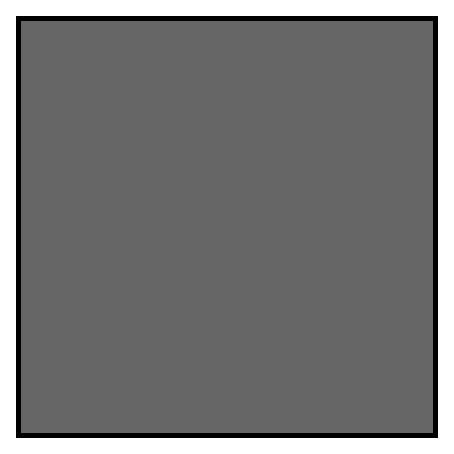
\includegraphics{example.eps}
%% figure caption is below the figure
%\caption{Please write your figure caption here}
%\label{fig:1}       % Give a unique label
%\end{figure}
%%
%% For two-column wide figures use
%\begin{figure*}
%% Use the relevant command to insert your figure file.
%% For example, with the graphicx package use
%  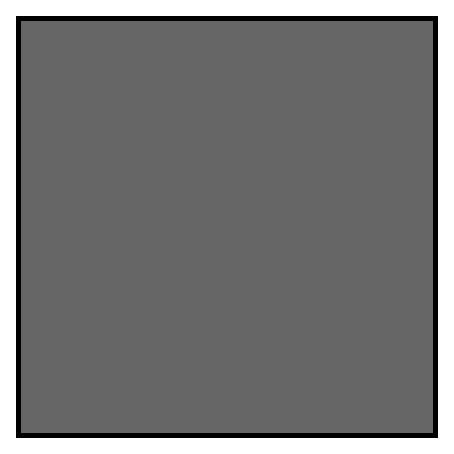
\includegraphics[width=0.75\textwidth]{example.eps}
%% figure caption is below the figure
%\caption{Please write your figure caption here}
%\label{fig:2}       % Give a unique label
%\end{figure*}
%%
%% For tables use
%\begin{table}
%% table caption is above the table
%\caption{Please write your table caption here}
%\label{tab:1}       % Give a unique label
%% For LaTeX tables use
%\begin{tabular}{lll}
%\hline\noalign{\smallskip}
%first & second & third  \\
%\noalign{\smallskip}\hline\noalign{\smallskip}
%number & number & number \\
%number & number & number \\
%\noalign{\smallskip}\hline
%\end{tabular}
%\end{table}


%\begin{acknowledgements}
%If you'd like to thank anyone, place your comments here
%and remove the percent signs.
%\end{acknowledgements}


% Authors must disclose all relationships or interests that 
% could have direct or potential influence or impart bias on 
% the work: 
%
% \section*{Conflict of interest}
%
% The authors declare that they have no conflict of interest.


% BibTeX users please use one of
%\bibliographystyle{spbasic}      % basic style, author-year citations
%\bibliographystyle{spmpsci}      % mathematics and physical sciences
%\bibliographystyle{spphys}       % APS-like style for physics
%\bibliography{}   % name your BibTeX data base

% Non-BibTeX users please use
\begin{thebibliography}{}

% and use \bibitem to create references. Consult the Instructions
% for authors for reference list style.
%
%\bibitem{RefJ}
% Format for Journal Reference
%Author, Article title, Journal, Volume, page numbers (year)
% Format for books
%\bibitem{RefB}
%Author, Book title, page numbers. Publisher, place (year)
% etc
\providecommand{\url}[1]{{#1}}
\providecommand{\urlprefix}{URL }
\expandafter\ifx\csname urlstyle\endcsname\relax
  \providecommand{\doi}[1]{DOI~\discretionary{}{}{}#1}\else
  \providecommand{\doi}{DOI~\discretionary{}{}{}\begingroup
  \urlstyle{rm}\Url}\fi

\bibitem{Absil2009}
Absil, P.A., Mahony, R., Sepulchre, R.: Optimization algorithms on matrix
  manifolds.
\newblock Princeton University Press, Princeton, NJ (2008).
\newblock \doi{10.1515/9781400830244}.
\newblock \urlprefix\url{http://dx.doi.org/10.1515/9781400830244}

\bibitem{Bertsekas2014}
Bertsekas, D.P.: Constrained optimization and {L}agrange multiplier methods.
\newblock Computer Science and Applied Mathematics. Academic Press, Inc.
  [Harcourt Brace Jovanovich, Publishers], New York-London (2014)

\bibitem{bortoloti2022efficient}
Bortoloti, M.A.A., Fernandes, T.A., Ferreira, O.P.: An efficient damped
  {N}ewton-type algorithm with globalization strategy on {R}iemannian
  manifolds.
\newblock J. Comput. Appl. Math. \textbf{403}, Paper No. 113853, 15 (2022).
\newblock \doi{10.1016/j.cam.2021.113853}.
\newblock \urlprefix\url{https://doi.org/10.1016/j.cam.2021.113853}

\bibitem{MR4102428}
Bortoloti, M.A.A., Fernandes, T.A., Ferreira, O.P., Yuan, J.: Damped {N}ewton's
  method on {R}iemannian manifolds.
\newblock J. Global Optim. \textbf{77}(3), 643--660 (2020).
\newblock \doi{10.1007/s10898-020-00885-0}.
\newblock \urlprefix\url{https://doi.org/10.1007/s10898-020-00885-0}

\bibitem{Burdakov1980}
Burdakov, O.: Some globally convergent modifications of Newton's method for
  solving systems of nonlinear equations.
\newblock In: Soviet mathematics-Doklady, vol.~22, pp. 376--378 (1980)

\bibitem{doCarmo1992}
do~Carmo, M.P.: Riemannian geometry.
\newblock Mathematics: Theory \& Applications. Birkh\"auser Boston, Inc.,
  Boston, MA (1992).
\newblock \doi{10.1007/978-1-4757-2201-7}.
\newblock \urlprefix\url{http://dx.doi.org/10.1007/978-1-4757-2201-7}.
\newblock Translated from the second Portuguese edition by Francis Flaherty

\bibitem{Dennis1996}
Dennis Jr., J.E., Schnabel, R.B.: Numerical methods for unconstrained
  optimization and nonlinear equations, \emph{Classics in Applied Mathematics},
  vol.~16.
\newblock Society for Industrial and Applied Mathematics (SIAM), Philadelphia,
  PA (1996).
\newblock \doi{10.1137/1.9781611971200}.
\newblock \urlprefix\url{http://dx.doi.org/10.1137/1.9781611971200}.
\newblock Corrected reprint of the 1983 original

\bibitem{FernandesAndFerreiraAndYuan2017}
Fernandes, T.A., Ferreira, O.P., Yuan, J.: On the {S}uperlinear {C}onvergence
  of {N}ewton's {M}ethod on {R}iemannian {M}anifolds.
\newblock J. Optim. Theory Appl. \textbf{173}(3), 828--843 (2017).
\newblock \doi{10.1007/s10957-017-1107-2}.
\newblock \urlprefix\url{http://dx.doi.org/10.1007/s10957-017-1107-2}

\bibitem{Ferreira2012}
Ferreira, O.P., Silva, R.C.M.: Local convergence of {N}ewton's method under a
  majorant condition in {R}iemannian manifolds.
\newblock IMA J. Numer. Anal. \textbf{32}(4), 1696--1713 (2012).
\newblock \doi{10.1093/imanum/drr048}.
\newblock \urlprefix\url{http://dx.doi.org/10.1093/imanum/drr048}

\bibitem{Luenberger1972}
Luenberger, D.G.: The gradient projection method along geodesics.
\newblock Management Sci. \textbf{18}, 620--631 (1972)

\bibitem{Manton2002}
Manton, J.H.: Optimization algorithms exploiting unitary constraints.
\newblock IEEE Trans. Signal Process. \textbf{50}(3), 635--650 (2002).
\newblock \doi{10.1109/78.984753}.
\newblock \urlprefix\url{https://doi.org/10.1109/78.984753}

\bibitem{Ortega1990}
Ortega, J.M.: Numerical analysis. {A} second course.
\newblock Academic Press, New York-London (1972).
\newblock Computer Science and Applied Mathematics

\bibitem{Sakai1996}
Sakai, T.: Riemannian geometry, \emph{Translations of Mathematical Monographs},
  vol. 149.
\newblock American Mathematical Society, Providence, RI (1996).
\newblock Translated from the 1992 Japanese original by the author

\bibitem{MR3734011}
Sato, H.: Riemannian {N}ewton-type methods for joint diagonalization on the
  {S}tiefel manifold with application to independent component analysis.
\newblock Optimization \textbf{66}(12), 2211--2231 (2017).
\newblock \doi{10.1080/02331934.2017.1359592}.
\newblock \urlprefix\url{https://doi.org/10.1080/02331934.2017.1359592}

\bibitem{sato2021}
Sato, H.: Riemannian Optimization and Its Applications.
\newblock Springer Nature (2021)


\end{thebibliography}
%\bibliographystyle{spphys}
%\bibliography{biblioGlobal}
%\bibliographystyle{spmpsci}
%\bibliography{biblioGlobal}

\end{document}
% end of file template.tex

